\documentclass[10pt,aspectratio=43,mathserif,table]{beamer} 
%设置为 Beamer 文档类型,设置字体为 10pt,长宽比为16:9,数学字体为 serif 风格
\batchmode

\usepackage{graphicx}
\usepackage{animate}
\usepackage{hyperref}


%导入一些用到的宏包
\usepackage{amsmath,bm,amsfonts,amssymb,enumerate,epsfig,bbm,calc,color,ifthen,capt-of,multimedia,hyperref}
\usepackage{xeCJK} %导入中文包
\setCJKmainfont{SimHei} %字体采用黑体  Microsoft YaHei

\usetheme{Berlin} %主题

\usepackage[ruled,linesnumbered]{algorithm2e}

\usepackage{fancybox}
\usepackage{xcolor}
\usepackage{times}
\usepackage{listings}

\usepackage{booktabs}
\usepackage{colortbl}

\newcommand{\Console}{Console}
\lstset{ %
	backgroundcolor=\color{white},   % choose the background color
	basicstyle=\footnotesize\rmfamily,     % size of fonts used for the code
	columns=fullflexible,
	breaklines=true,                 % automatic line breaking only at whitespace
	captionpos=b,                    % sets the caption-position to bottom
	tabsize=4,
	commentstyle=\color{mygreen},    % comment style
	escapeinside={\%*}{*)},          % if you want to add LaTeX within your code
	keywordstyle=\color{blue},       % keyword style
	stringstyle=\color{mymauve}\ttfamily,     % string literal style
	numbers=left, 
	%	frame=single,
	rulesepcolor=\color{red!20!green!20!blue!20},
	% identifierstyle=\color{red},
	language=c
}


\definecolor{mygreen}{rgb}{0,0.6,0}
\definecolor{mymauve}{rgb}{0.58,0,0.82}
\definecolor{mygray}{gray}{.9}
\definecolor{mypink}{rgb}{.99,.91,.95}
\definecolor{mycyan}{cmyk}{.3,0,0,0}

%题目,作者,学校,日期
\title{Application of dfs order to graph theory problems}
\subtitle{\fontsize{9pt}{14pt}\textbf{dfs序在图论问题的应用}}
\author{主讲: 赵涵铮}
\institute{agile studio}
\date{\today}

%学校Logo
%\pgfdeclareimage[height=0.5cm]{sustech-logo}{sustech-logo.pdf}
%\logo{\pgfuseimage{sustech-logo}\hspace*{0.3cm}}

\AtBeginSection[]
{
	\begin{frame}<beamer>
		\frametitle{\textbf{目录}}
		\tableofcontents[currentsection]
	\end{frame}
}
\beamerdefaultoverlayspecification{<+->}
% -----------------------------------------------------------------------------
\begin{document}
	% -----------------------------------------------------------------------------
	
	\frame{\titlepage}
	
	\section[目录]{}   %目录
	\begin{frame}{目录}
		\tableofcontents
	\end{frame}
	
	% -----------------------------------------------------------------------------
	\section{引言}  %引言
	\begin{frame}{DFS序列简介}
		\begin{block}{DFS 序列}
			DFS 序列是指 DFS 调用过程中访问的节点编号的序列。
			
			一个显而易见的性质就是,每个子树都对应 DFS 序列中的连续一段(一段区间)。
		\end{block}
		用巧妙的深搜,去化解复杂的图。
	\end{frame}
	
	\section{例题}
	\subsection{汽车老板}
	\begin{frame}{\href{https://www.mfstem.org/p/1559}{汽车老板}}
		
		\begin{block}{题意}
			给定一棵树,共$M$次操作,每次操作:
			
			1.使得一个节点$a$的所有子孙节点的值加$x$。
			
			2.求节点$a$的值。
		\end{block}
	\end{frame}
	
	\begin{frame}
		此树的dfs序为:1,3,4,5,2,可以想到,每个子树都对应 DFS 序列中的连续一段,那么对子树操作就等同于对于区间操作。
		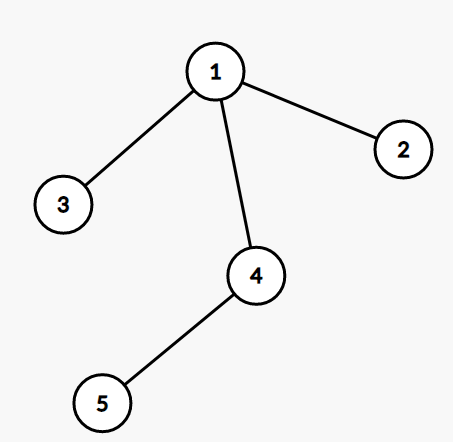
\includegraphics[width = 0.65\linewidth]{./figure/tree}		
	\end{frame}
	
	\subsection{Cycling City}
	\begin{frame}{\href{https://codeforces.com/problemset/problem/521/E}{Cycling City}}
		\begin{block}{题目大意}
			给定一张图,询问是否有两个点,使得两个点有三条路,且这三条路没有公共点。
			$$n,m\leq 2*10^5$$
		\end{block}
	\end{frame}
	
	\begin{frame}
		通过dfs,可以将一张图分解成树和返祖边
		
		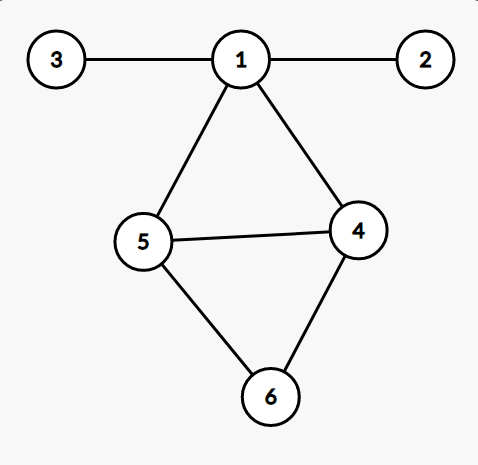
\includegraphics[width = 0.4\linewidth]{./figure/before}		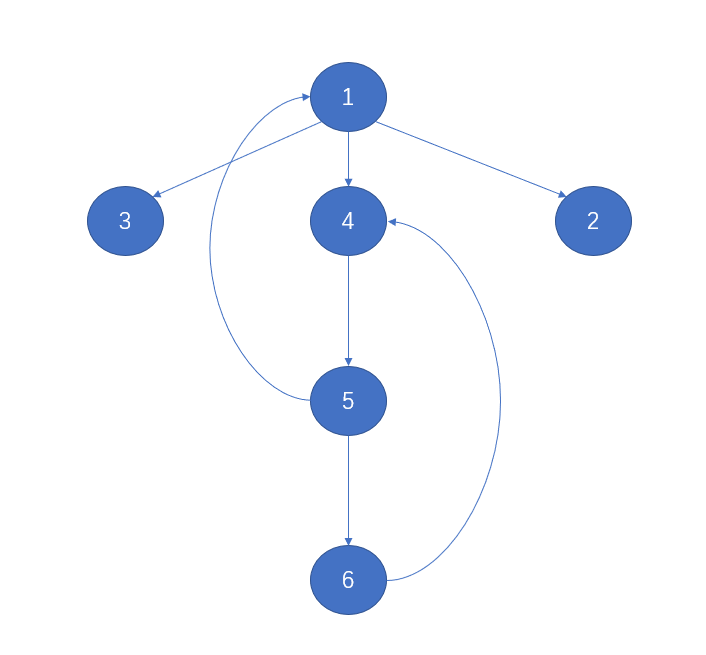
\includegraphics[width = 0.4\linewidth]{./figure/after}		
	\end{frame}
	
	\subsection{Cycle}
	\begin{frame}{\href{https://acm.hdu.edu.cn/showproblem.php?pid=5215}{Cycle}}
		\begin{block}{题目大意}
			给定一张图,询问是否有两个点,使得两个点有三条路,且这三条路没有公共点。
			$$n\leq 10^5,m\leq 3*10^5$$
		\end{block}
	\end{frame}
	
	\begin{frame}
		来想一想两个环如何组合?
	
		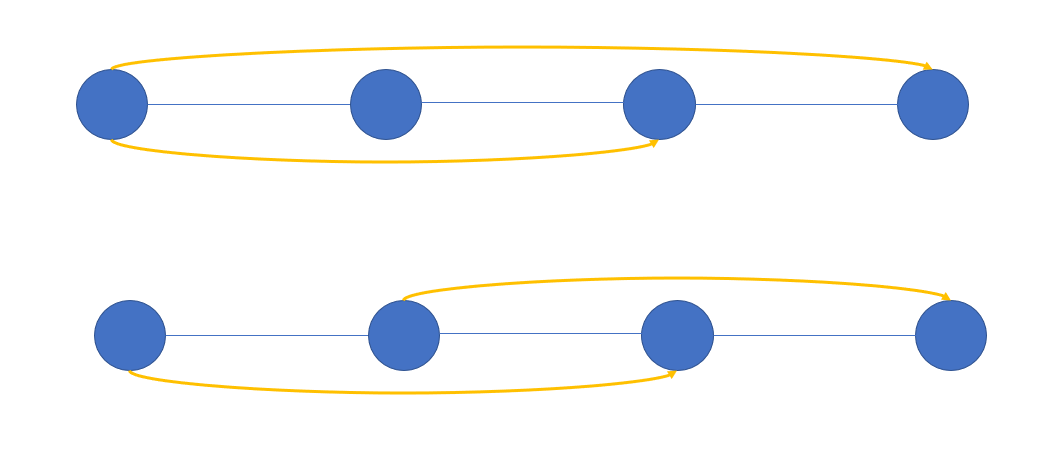
\includegraphics[width = 0.9\linewidth]{./figure/cycle}		
	\end{frame}
	
	\section{结语}
	\begin{frame}{Thank you}
		\begin{center}
			\begin{minipage}{1\textwidth}
				\setbeamercolor{mybox}{fg=white, bg=black!50!blue}
				\begin{beamercolorbox}[wd=0.70\textwidth, rounded=true, shadow=true]{mybox}
					\LARGE \centering Thank you for listening!  %结束语
				\end{beamercolorbox}
			\end{minipage}
		\end{center}
	\end{frame}
	
	\begin{frame}{Q\&A}
		\begin{center}
			\begin{minipage}{1\textwidth}
				\setbeamercolor{mybox}{fg=white, bg=black!50!blue}
				\begin{beamercolorbox}[wd=0.70\textwidth, rounded=true, shadow=true]{mybox}
					\LARGE \centering  Questions?  %请求提问
				\end{beamercolorbox}
			\end{minipage}
		\end{center}
	\end{frame}
	
	% -----------------------------------------------------------------------------
\end{document}
%文档结束